\section{paleoTS}

\subsubsection*{Europe, genera, continental}\label{europe-genera-continental}

\begin{longtable}[]{@{}rrrr@{}}
	\caption{paleoTs object, Europe, continental}
	\label{tab:pTSEuC}\tabularnewline
	\toprule
	mm & nn & vv & tt\tabularnewline
	\midrule
	\endfirsthead
	\toprule
	mm & nn & vv & tt\tabularnewline
	\midrule
	\endhead
	149.5381 & 2 & 3450.8267 & 0.00585\tabularnewline
	187.0000 & 1 & 0.0000 & 0.06885\tabularnewline
	205.4750 & 2 & 198.0050 & 0.45350\tabularnewline
	204.9292 & 2 & 23.1767 & 1.29350\tabularnewline
	1420.0000 & 1 & 0.0000 & 2.19700\tabularnewline
	232.5000 & 1 & 0.0000 & 3.09400\tabularnewline
	1475.6667 & 3 & 57926.3333 & 4.46600\tabularnewline
	663.3750 & 2 & 473607.7812 & 6.28900\tabularnewline
	800.0508 & 6 & 263434.3893 & 9.42700\tabularnewline
	653.9625 & 5 & 351634.5281 & 12.71400\tabularnewline
	772.0000 & 5 & 223154.3750 & 14.89500\tabularnewline
	533.8533 & 5 & 183706.6821 & 19.50000\tabularnewline
	\bottomrule
\end{longtable}

\begin{figure}[H]
	\centering
	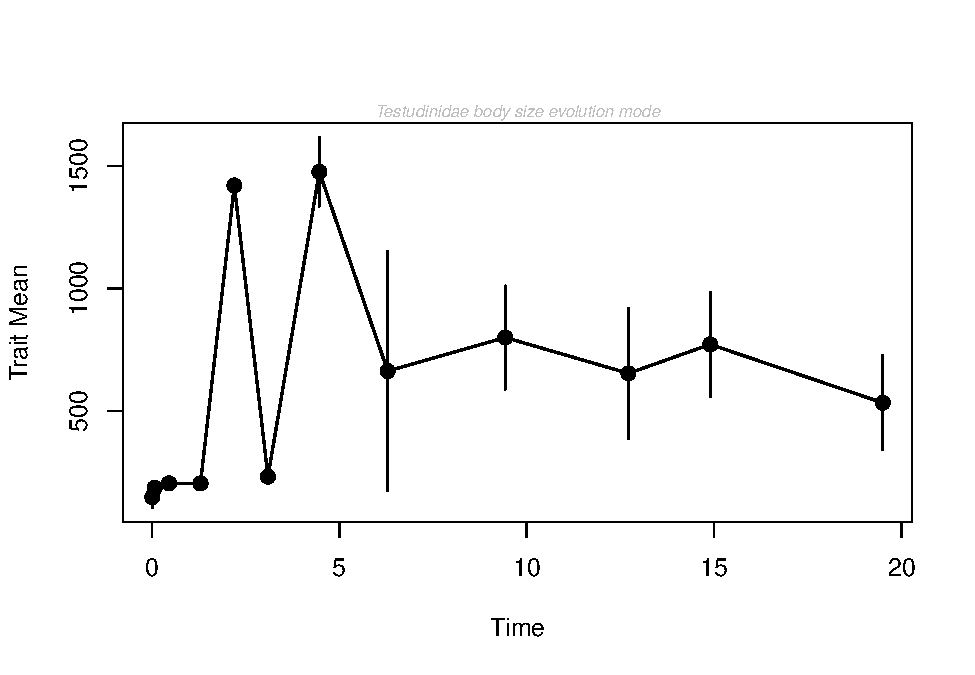
\includegraphics{MA_JJ_files/figure-latex/pTSEuC-1.pdf}
	\caption{paleoTS, genera, Europe, continental}
	\label{fig:pTSEuC}
\end{figure}

\begin{longtable}[]{@{}lrrrr@{}}
	\caption{Model-fitting results for testudinidae, genera, Europe,
		continental}
	\label{tab:pTSEuCEM}\tabularnewline
	\toprule
	& logL & K & AICc & Akaike.wt\tabularnewline
	\midrule
	\endfirsthead
	\toprule
	& logL & K & AICc & Akaike.wt\tabularnewline
	\midrule
	\endhead
	GRW & -87.93137 & 2 & 181.3627 & 0.009\tabularnewline
	URW & -92.56882 & 1 & 187.5821 & 0.000\tabularnewline
	Stasis & -83.21073 & 2 & 171.9215 & 0.991\tabularnewline
	\bottomrule
\end{longtable}


\FloatBarrier

%__________________________________________________________________________


\subsubsection*{Europe, genera,
	insular}\label{europe-genera-insular}

\begin{longtable}[]{@{}rrrr@{}}
	\caption{paleoTs object, Europe, insular}
	\label{tab:pTSEuI}\tabularnewline
	\toprule
	mm & nn & vv & tt\tabularnewline
	\midrule
	\endfirsthead
	\toprule
	mm & nn & vv & tt\tabularnewline
	\midrule
	\endhead
	187.5077 & 1 & 0.00 & 0.00585\tabularnewline
	831.5000 & 2 & 684.50 & 0.06885\tabularnewline
	722.5000 & 1 & 0.00 & 0.45350\tabularnewline
	835.0833 & 4 & 168423.36 & 1.29350\tabularnewline
	1005.0000 & 2 & 1462050.00 & 2.19700\tabularnewline
	451.6667 & 3 & 40558.33 & 3.09400\tabularnewline
	826.1667 & 2 & 15196.06 & 4.46600\tabularnewline
	1850.0000 & 1 & 0.00 & 6.28900\tabularnewline
	\bottomrule
\end{longtable}

\begin{figure}[H]
	\centering
	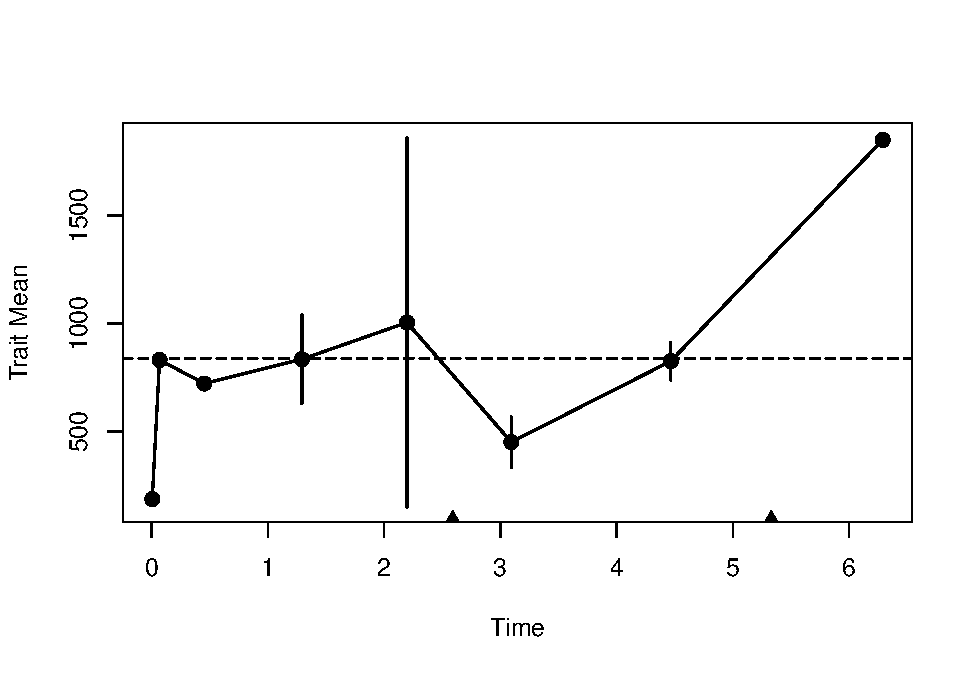
\includegraphics{MA_JJ_files/figure-latex/pTSEuI-1.pdf}
	\caption{paleoTS, genera, Europe, insular}
	\label{fig:pTSEuI}
\end{figure}

\begin{longtable}[]{@{}lrrrr@{}}
	\caption{Model-fitting results for testudinidae, genera, Europe,
		insular}
	\label{tab:pTSEuIEM}\tabularnewline
	\toprule
	& logL & K & AICc & Akaike.wt\tabularnewline
	\midrule
	\endfirsthead
	\toprule
	& logL & K & AICc & Akaike.wt\tabularnewline
	\midrule
	\endhead
	GRW & -67.12192 & 2 & 141.2438 & 0.000\tabularnewline
	URW & -57.51634 & 1 & 117.8327 & 0.074\tabularnewline
	Stasis & -52.89638 & 2 & 112.7928 & 0.926\tabularnewline
	\bottomrule
\end{longtable}

\FloatBarrier
%_________________________________________________________________________




\subsubsection*{Eurasia, genera,
	continental}\label{eurasiagenera-continental}

\begin{longtable}[]{@{}rrrr@{}}
	\caption{paleoTS object, all data}\tabularnewline
	\toprule
	mm & vv & nn & tt\tabularnewline
	\midrule
	\endfirsthead
	\toprule
	mm & vv & nn & tt\tabularnewline
	\midrule
	\endhead
	210.8687 & 10460.89 & 6 & 0.00585\tabularnewline
	530.0000 & 122579.33 & 4 & 0.06885\tabularnewline
	377.8167 & 89203.95 & 3 & 0.45350\tabularnewline
	777.5579 & 162641.14 & 7 & 1.29350\tabularnewline
	909.6667 & 562217.22 & 5 & 2.19700\tabularnewline
	892.0000 & 381770.00 & 5 & 3.09400\tabularnewline
	1048.0556 & 296417.22 & 6 & 4.46600\tabularnewline
	1208.9167 & 849651.02 & 3 & 6.28900\tabularnewline
	800.0508 & 263434.39 & 6 & 9.42700\tabularnewline
	653.9625 & 351634.53 & 5 & 12.71400\tabularnewline
	772.0000 & 223154.38 & 5 & 14.89500\tabularnewline
	513.8533 & 162399.35 & 5 & 19.50000\tabularnewline
	\bottomrule
\end{longtable}

\begin{figure}[H]
	\centering
	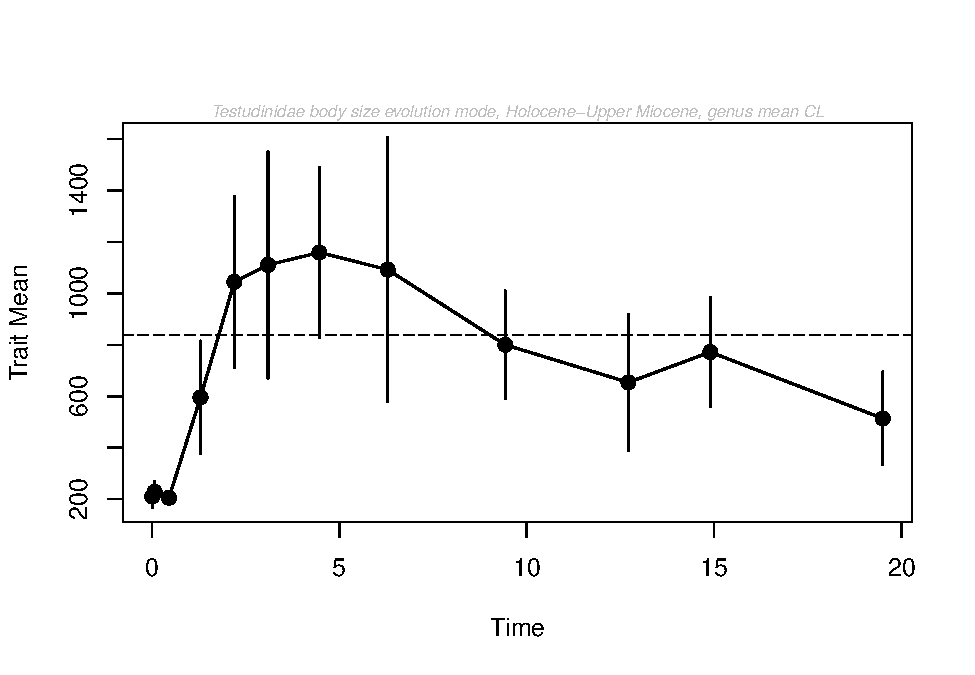
\includegraphics{MA_JJ_files/figure-latex/pTSEsC-1.pdf}
	\caption{paleoTS, genera, Eurasia, continental}
	\label{fig:pTSEsC}
\end{figure}

\begin{longtable}[]{@{}lrrrr@{}}
	\caption{Model-fitting results for testudinidae, genera, Eurasia,
		continental}
	\label{tab:pTSEsC}
	\tabularnewline
	\toprule
	& logL & K & AICc & Akaike.wt\tabularnewline
	\midrule
	\endfirsthead
	\toprule
	& logL & K & AICc & Akaike.wt\tabularnewline
	\midrule
	\endhead
	GRW & -74.89025 & 2 & 155.2805 & 0.211\tabularnewline
	URW & -75.10165 & 1 & 152.6477 & 0.787\tabularnewline
	Stasis & -79.85118 & 2 & 165.2024 & 0.001\tabularnewline
	\bottomrule
\end{longtable}


\FloatBarrier
%__________________________________________________________________________

\subsubsection*{Eurasia, genera,
	insular}\label{eurasiagenera-insular}

\begin{longtable}[]{@{}rrrr@{}}
	\caption{paleoTS object, all data}\tabularnewline
	\toprule
	mm & vv & nn & tt\tabularnewline
	\midrule
	\endfirsthead
	\toprule
	mm & vv & nn & tt\tabularnewline
	\midrule
	\endhead
	230.9239 & 10020.53 & 5 & 0.00585\tabularnewline
	644.3333 & 105436.33 & 3 & 0.06885\tabularnewline
	722.5000 & 0.00 & 1 & 0.45350\tabularnewline
	882.0356 & 105684.08 & 6 & 1.29350\tabularnewline
	953.6667 & 652233.89 & 5 & 2.19700\tabularnewline
	891.0000 & 383430.00 & 5 & 3.09400\tabularnewline
	620.4444 & 134562.93 & 3 & 4.46600\tabularnewline
	1900.0000 & 5000.00 & 2 & 6.28900\tabularnewline
	800.0000 & 0.00 & 1 & 19.50000\tabularnewline
	\bottomrule
\end{longtable}

\newpage

\begin{figure}[H]
	\centering
	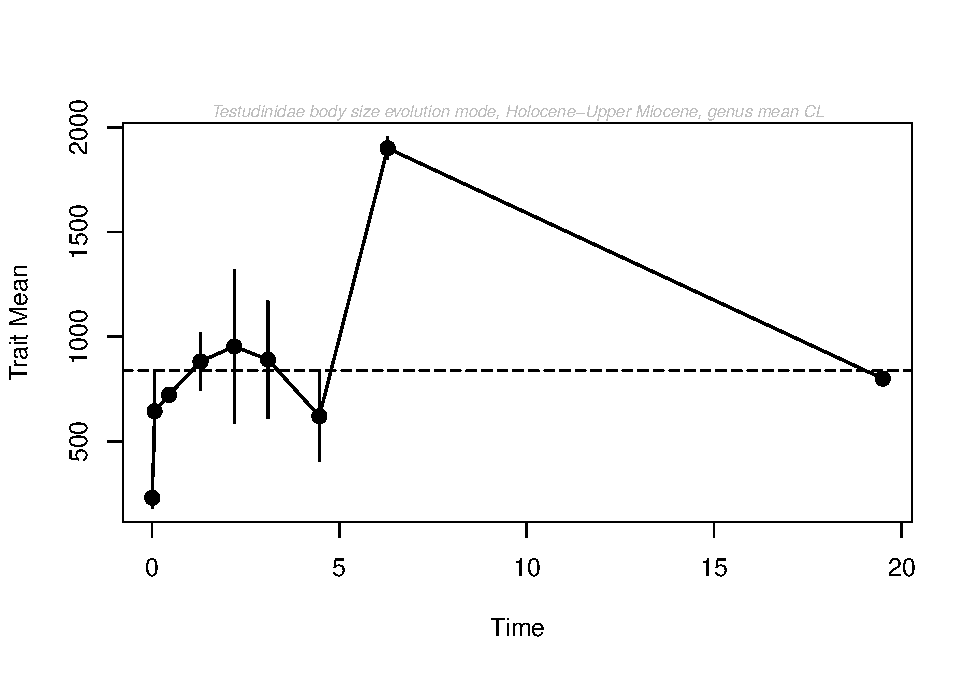
\includegraphics{MA_JJ_files/figure-latex/pTSEsI-1.pdf}
	\caption{paleoTS, genera, Eurasia, insular}
	\label{fig:pTSEsI}
\end{figure}

\begin{longtable}[]{@{}lrrrr@{}}
	\caption{Model-fitting results for testudinidae, genera, Eurasia,
		insular}
	\label{tab:pTSEsI}
	\tabularnewline
	\toprule
	& logL & K & AICc & Akaike.wt\tabularnewline
	\midrule
	\endfirsthead
	\toprule
	& logL & K & AICc & Akaike.wt\tabularnewline
	\midrule
	\endhead
	GRW & -61.85159 & 2 & 130.1032 & 0.070\tabularnewline
	URW & -62.38003 & 1 & 127.4267 & 0.265\tabularnewline
	Stasis & -59.59249 & 2 & 125.5850 & 0.666\tabularnewline
	\bottomrule
\end{longtable}


\FloatBarrier






